

% \begin{figure}[h]
% 
\includegraphics[width=\linewidth]{img/warning.png}
% % \caption{A boat.}
% % \label{fig:boat1}
% \end{figure}
% Figure \ref{fig:boat1} shows a boat.

% \warningbeg % ПРАВИТЬ!
Введение нужно написать в самом конце. \\
Пока что тут будет просто план:        \\
- Что то про развитие (электромобили, беплы)  \\
- Про необходимость балансировки  \\
- Что нибудь ещё \\
Для справки
% Собснаа все по госту(нет)
\begin{figure}[h]
    \fbox{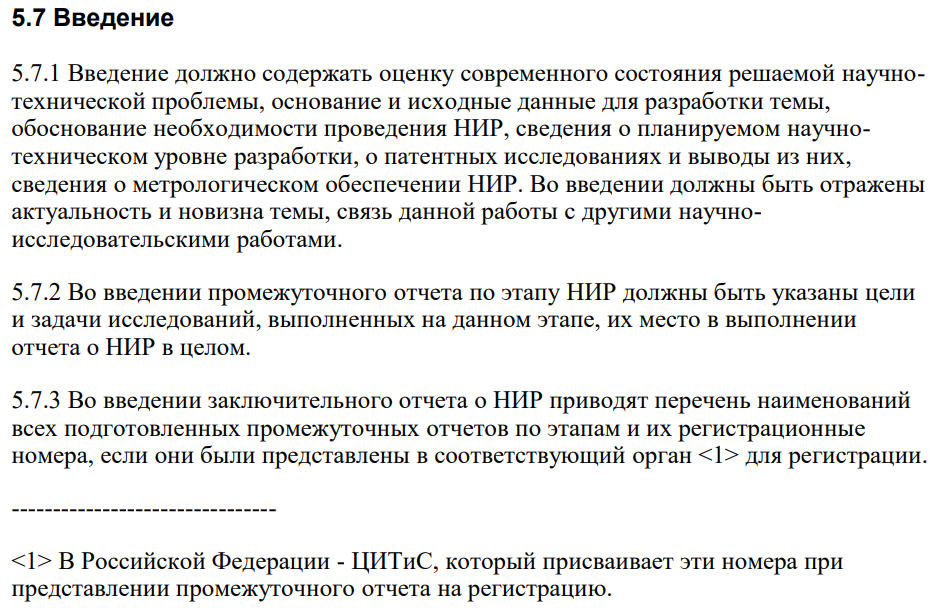
\includegraphics[width=420px]{img/dev/GOST_intro.png}}
\end{figure}

% \warningend % ПРАВИТЬ!
\newpage

% За последние 20 лет появилось огромное количество
% На сегодняшний день известно множевство различных аккумуляторных элементов

% К сожалению электродвигатели уступают по удельной мощности жидкостнотопливным реактивным и поршневым \aca{su}. 
% В качестве примера подойдёт проект NASA X-57 ''Maxwell''

% Rotax 912S3 
% Мощность:  2 × 100 л.с..
% Резюмируя вышесказанное - наиболее используемые литий-полимерные аккумуляторы сильно уступают существующим \aca{su}.
% Однако не стоит недооценивать важность \aca{bms} для авиастроениия. Подобную систему контроля можно использовать и с другими типами ... , например суперкондестаторы
% Возможно в будущем будут открыты 'тёплые' сверхпроводники, что позволит увеличить удельную мощность электродвигателей в n раз (см. Источник)  
% По этому данный материал стоит рассматривать не более чем научно-технический задел

